\chapter{Methodology}
\section{Object Detection Architectures and Backbones}
\label{sec:arch_and_backbones}
The core of our lung nodule detection pipeline is built upon a robust and well-established object detection framework. For this research, experiments will be conducted on the architectures discussed in the previous chapter: Faster R-CNN and RetinaNet.

While these architectures defines the overall detection process, the quality of the features extracted from the input image is can impact its success. This feature extraction is performed by a deep convolutional neural network, commonly referred to as the backbone. The choice of backbone directly influences the model's performance, computational complexity, and memory footprint. A central component of our methodology is therefore to systematically evaluate the impact of different backbone architectures on the lung nodule detection task.

To investigate the trade-off between model performance and computational efficiency, we conducted experiments with three distinct backbone architectures, each representing a different design philosophy:

\begin{itemize}
    \item \textbf{ResNet50:} A canonical and widely adopted architecture, ResNet50 serves as a robust and powerful baseline. Its use of residual connections allows for the effective training of very deep networks, making it a standard choice for a vast range of computer vision tasks. With 25.5 million parameters, it represents a high-performance, but computationally intensive, option.

    \item \textbf{MobileNetV2:} Designed specifically for efficiency and deployment on resource constrained devices, MobileNetV2 is a lightweight architecture with only 5.4 million parameters. It utilizes inverted residual blocks and linear bottlenecks to achieve a favorable balance between accuracy and computational cost, making it an ideal candidate for exploring the feasibility of more accessible clinical tools.

    \item \textbf{EfficientNetV2-S:} This model represents a modern approach to network design, seeking to optimally balance accuracy, training speed, and parameter efficiency. By systematically scaling network depth, width, and resolution, and employing novel architectural blocks, EfficientNetV2-S (with 21.4 million parameters) offers performance competitive with larger models while maintaining a smaller computational footprint.
\end{itemize}

In all experiments, each backbone was initialized with weights pre-trained on the ImageNet1k dataset. This transfer learning approach is a standard practice that leverages the rich, hierarchical features learned from a large-scale, general-purpose dataset to significantly improve performance and reduce training time on smaller, specialized datasets such as the one used in this study. 

\subsection{Loss functions}
\label{sec:loss_functions}
A central metric for bounding box quality is the \textit{Intersection over Union} (IoU):
$$
\mathrm{IoU}(b, b^\ast) = \frac{\mathrm{area}(b \cap b^\ast)}{\mathrm{area}(b \cup b^\ast)},
$$
which measures the degree of spatial overlap between a predicted box $b$ and a ground-truth box $b^\ast$.
Variants such as Generalized IoU (GIoU), Distance IoU (DIoU), and Complete IoU (CIoU) incorporate additional geometric terms to improve optimization stability, particularly when boxes do not overlap \cite{rezatofighi2019giou,zheng2019diou, zheng2021ciou}.


Bounding box regression is also commonly evaluated in coordinate space using Minkowski distances.
The general $p$-norm between two vectors $u,v \in \mathbb{R}^n$ is defined as:
$$
\| u - v \|_p = \left( \sum_{j=1}^n |u_j - v_j|^p \right)^{\frac{1}{p}}.
$$
Special cases include the Manhattan distance ($L_1$ norm, $p=1$):
$$
\| u - v \|_1 = \sum_{j=1}^n |u_j - v_j|,
$$
and the Euclidean distance ($L_2$ norm, $p=2$):
$$
\| u - v \|_2 = \sqrt{\sum_{j=1}^n (u_j - v_j)^2}.
$$

In practice, modern detectors often adopt the Smooth-$L_1$ loss \cite{girshick2015fastrcnn} for bounding box regression, which combines the robustness of $L_1$ for large errors with the stability of $L_2$ for small errors:
$$
\mathrm{SmoothL1}(x) =
\begin{cases}
0.5\,x^2, & \text{if } |x| < 1, \\
|x| - 0.5, & \text{otherwise}.
\end{cases}
$$
This formulation reduces sensitivity to outliers while maintaining differentiability at the origin, making it suitable for gradient-based optimization.

As for the classification component, Faster R-CNN employs the standard cross-entropy loss for binary classification tasks, while RetinaNet utilizes the Focal Loss \cite{lin2018focalloss} to address class imbalance by down-weighting easy negatives and focusing training on hard examples.

\section{Object Detection Data Preprocessing}
\subsection{Train-time Augmentations}
\label{sec:augmentation}
To further enhance the robustness of our models and improve their generalization capabilities, we apply a series of data augmentations during training. These augmentations include random rotations, flips, and intensity variations, which help to simulate the variability encountered in real-world clinical settings. By exposing the model to a diverse set of augmented images, we aim to reduce overfitting and improve the model's ability to generalize to unseen data. These augmentations are applied on-the-fly during training, ensuring that the model sees a different version of the data in each epoch.

The specific augmentations applied are as follows:
\begin{itemize}
    \item \textbf{Horizonal Flips}: Each image has a 50\% chance of being flipped horizontally. This augmentation helps the model learn invariance to left-right orientation, which is particularly relevant in medical imaging where anatomical structures can appear in various orientations.
    \item \textbf{Shift, Scale and Rotate}: Each image has a 50\% change of being randomly shifted (up to 5\% of image dimensions), scaled (between 0.9 and 1.1 times the original size), and rotated (up to 15 degrees). These transformations simulate variations in patient positioning and imaging angles, enhancing the model's ability to recognize nodules under different conditions.
    \item \textbf{Random Brightness and Contrast}: Each image has a 50\% chance of having its brightness and contrast randomly adjusted. Brightness is modified by a factor between -0.1 and +0.1, while contrast is adjusted by a factor between 0.9 and 1.1. This augmentation accounts for differences in imaging protocols and equipment, helping the model to generalize across varying image qualities.
    \item \textbf{CLAHE (Contrast Limited Adaptive Histogram Equalization)}: \\Each image has a 50\% chance of being processed with CLAHE. This technique enhances local contrast and improves the visibility of structures in areas that are too dark or too bright, which is particularly useful in medical images where subtle features can be critical for diagnosis \cite{mishra2021clahe}.
\end{itemize}


\section{Object Detection Pipeline}
To synthesize the previously described components, this section outlines the complete, end-to-end workflow used for training and evaluating the lung nodule detection models. This systematic process ensures reproducibility and provides a clear framework for the experiments presented in this thesis. The workflow proceeds in three main stages:

\begin{enumerate}
    \item \textbf{Data Preparation.} The initial raw 3D CT volumes from the DLCS dataset are processed through a sequential pipeline to generate the final training data:
    \begin{itemize}
        \item Each CT volume is first resampled to a uniform voxel spacing (Section \ref{sec:resampling}).
        \item 2D axial slices are extracted from each 3D volumetric annotation.
        \item The resulting set of slices is filtered using the Informed HU Thresholding strategy to reduce annotation noise (Section \ref{sec:dataset_pruning}).
        \item Finally, the 2.5D three-channel input representation is constructed for each target slice (Section \ref{sec:2.5d_approach}).
    \end{itemize}

    \item \textbf{Model Training.} The Faster R-CNN/RetinaNet model is trained on the prepared dataset. 
    \begin{itemize}
        \item The impact of different backbone architectures (ResNet50, MobileNetV2, EfficientNetV2-S) is systematically evaluated (Section \ref{sec:arch_and_backbones}).
        \item The training process incorporates extensive online data augmentation (Section \ref{sec:augmentation}) to prevent overfitting and is guided by a consistent set of hyperparameters (AdamW optimizer, Cosine Annealing scheduler).
    \end{itemize}

    \item \textbf{Evaluation.} The trained models are evaluated on a held-out test set. 
    \begin{itemize}
        \item The models' predictions are compared against the ground truth annotations.
        \item Performance is quantitatively measured using the standard COCO metrics of Mean Average Precision (mAP) and Mean Average Recall (mAR), as formally defined in Section \ref{sec:eval_metrics}.
    \end{itemize}
\end{enumerate}


\section{Classification Head Module}
% Discuss the classification network, how we extracted a classification dataset from the detection dataset using the bounding boxes. 

The classification head is a detached component that builds learns to classify individual lung nodules as benign or malignant.
We decided to implement this as a separate model for several reasons:
A separate classification head introduces both modularity and flexibility, since it can be developed, tested, and optimized independently of the detection model. This separation makes it easier to experiment with alternative architectures and hyperparameters without interfering with the detection component. At the same time, isolating the classification task allows for greater specialization. Unlike detection, classification comes with its own requirements and challenges; by decoupling the two, the architecture and training process can be tailored specifically to the subtleties of distinguishing between benign and malignant nodules.
Finally, a separate classification head allows for a separate XAI analysis, allowing us to focus on explaining the classification decision independently of the detection process.

\subsection{Models and Training Procedure}
Since each data sample at our disposal inherently provides low information due to its small size, we opted for lightweight architectures to mitigate overfitting risks.
Specifically we experimented with:
\begin{itemize}
    \item \textbf{EfficientNetV2-S:} A modern architecture that balances performance and efficiency, making it suitable for tasks with limited data \cite{tan2020efficientnet}.
    \item \textbf{MobileNetV2:} Known for its lightweight design, MobileNetV2 is optimized for mobile and embedded applications, making it a good fit for scenarios where computational resources are constrained \cite{sandler2019mobilenetv2}.
    \item \textbf{ResNet18:} A shallower variant of the ResNet family, which retains the benefits of residual connections while being less prone to overfitting on small datasets \cite{he2015resnet}.
    \item \textbf{DenseNet121:} A compact architecture that promotes feature reuse through dense connections, which can be beneficial for learning from limited data \cite{huang2018densenet121}.
    \item \textbf{ConvNeXt-Tiny:} A modern architecture that incorporates design principles from both CNNs and Transformers, offering a balance between performance and efficiency \cite{liu2022convnext}.
\end{itemize}
To each of these architectures, we appended a custom classification head described in Table \ref{tab:classification-head}. This head consists of a series of fully connected layers interleaved with Layer Normalization, SiLU activation functions \cite{elfwing2017silu}, and Dropout for regularization. The final layer outputs logits corresponding to the two classes.

\begin{table}[h]
    \centering
    \begin{tabular}{|c|c|c|}
    \hline
    \textbf{Layer} & \textbf{Input $\rightarrow$ Output} & \textbf{Details} \\
    \hline
    Linear & in\_features $\rightarrow$ 256 & Fully connected layer \\
    LayerNorm & 256 & Normalization \\
    SiLU & 256 & Activation \\
    Dropout & 256 & $p=0.25$ \\
    \hline
    Linear & 256 $\rightarrow$ 512 & Fully connected layer \\
    LayerNorm & 512 & Normalization \\
    SiLU & 512 & Activation \\
    Dropout & 512 & $p=0.25$ \\
    \hline
    Linear & 512 $\rightarrow$ 512 & Fully connected layer \\
    LayerNorm & 512 & Normalization \\
    SiLU & 512 & Activation \\
    Dropout & 512 & $p=0.25$ \\
    \hline
    Linear & 512 $\rightarrow$ num\_classes & Output classifier \\
    \hline
    \end{tabular}
    \caption{Architecture of the classification head.}
    \label{tab:classification-head}
\end{table}
    
All models were initialized with weights pre-trained on ImageNet1k and fine-tuned on our lung nodule classification dataset. The training process utilized the Adam optimizer \cite{kingma2017adam} with a learning rate of $1e^{-4}$, a batch size of 8, and a harsh weight decay of $1e^{-3}$. A cosine annealing learning rate scheduler was employed to adjust the learning rate dynamically during training. The Focal Loss function was used to guide the optimization process, reflecting the binary nature of the classification task.

\subsection{Train-time Augmentations}
To enhance the robustness and generalization capabilities of our classification models, we applied a series of data augmentations during training. These augmentations are designed to simulate the variability encountered in real-world clinical settings, thereby reducing overfitting and improving the model's ability to generalize to unseen data. The specific augmentations applied are as follows:
\begin{itemize}
    \item Horizontal \& Vertical Flips: Each image has a 50\% chance of being flipped horizontally and a 50\% chance of being flipped vertically. This augmentation helps the model learn invariance to orientation, which is particularly relevant in medical imaging where anatomical structures can appear in various orientations.
    \item Random Brightness and Contrast: Each image has a 50\% chance of having its brightness and contrast randomly adjusted. Brightness is modified by a factor between -0.1 and +0.1, while contrast is adjusted by a factor between 0.9 and 1.1. This augmentation accounts for differences in imaging protocols and equipment, helping the model to generalize across varying image qualities.
    \item Contrast Limited Adaptive Histogram Equalization (CLAHE): Each image has a 30\% chance of being processed with CLAHE. This technique enhances local contrast and improves the visibility of structures in areas that are too dark or too bright, which is particularly useful in medical images where subtle features can be critical for diagnosis \cite{mishra2021clahe}.
    \item Center shifting: Each image gets randomly shifted of $\pm 5$ pixels in both and y directions. This augmentation simulates slight misalignments that can occur during image acquisition, helping the model to become more robust to positional variations.
\end{itemize}

\section{Explainability Methods}
% Describe how are we using the adapted CAM methods, which layers we're targeting and an example of expected output.
% Explain how we're going to compare the explainability methods using the distance game.
\label{sec:xai_methods}

To provide insight into the model's decision-making process we employ several gradient-free Class Activation Map (CAM) methods. As established in Chapter \ref{ch:background}, gradient-free methods are necessary to circumvent the challenges posed by the structured outputs and non-differentiable operations (e.g., NMS) inherent to the Faster R-CNN architecture. Specifically, we implement and evaluate three adapted CAM techniques: Eigen-CAM, Score-CAM, and Smoothed Score-CAM (SS-CAM).

\subsection{CAM Implementation and Application}
\label{subsec:cam_implementation}

The generation of a CAM explanation requires targeting a specific layer within the network from which to extract activation maps. For all CAM methods used in this work, in this study cases it is usual to select the final feature map produced by the Feature Pyramid Network (FPN) component. This layer contains rich semantic information but at a reduced spatial resolution. To account for this, we compute the CAM also at the second to last FPN layer, which has a higher spatial resolution but less semantic abstraction. 
Finally, we average the two resulting heatmaps once they have been upsampled to the original input size.

The process for generating an explanation for a given input image is as follows:
\begin{enumerate}
    \item The input image is passed through the model to obtain the baseline predictions (bounding boxes, labels, and scores).
    \item The chosen CAM method (Eigen-CAM, Score-CAM, or SS-CAM) is then applied, using the activations from the target FPN layer. For Score-CAM and SS-CAM, this involves the adapted \texttt{FasterRCNNBoxScoreTarget} function to handle the object detection outputs.
    \item The output is a 2D saliency map, or heatmap, of the same dimensions as the input slice.
\end{enumerate}

The expected output is an interpretable visualization. To produce this, the raw heatmap is normalized to the range $[0, 1]$, color-mapped (typically from blue for low activation to red for high activation), and overlaid with transparency on the original CT slice. This visualization directly highlights the pixels and regions the model found most salient when making its detection decision.

\subsection{Quantitative Evaluation of CAM Methods}
\label{subsec:xai_evaluation}

A purely visual inspection of heatmaps is subjective and insufficient for a rigorous comparison of explainability methods. To objectively and quantitatively compare the faithfulness of the different CAM techniques, there are several established "games" or evaluation protocols in the literature \cite{selvaraju2019gradcam,chattopadhay_2018gradcam++,wang2020score}. In this work, we noticed a significant amount of noise in the generated heatmaps, likely due to the inherent complexity of the detection task and the scarcity of annotated data.
To mitigate this, we designed and implemented a novel evaluation protocol called the "\textit{Inverse Distance Game}", inspired by the "Segmentation Game" proposed in \cite{chattopadhay_2018gradcam++}.

The goal of this game is to measure how well the close are the highest activation scores of a CAM's explanation are to the actual, ground-truth location of the nodule. To do so we proceed as described in Algorithm \ref{alg:distance-game}.

\begin{algorithm}[H]
    \caption{The Inverse Distance Game}
    \label{alg:distance-game}
    \DontPrintSemicolon
    \SetAlgoLined
    \setstretch{1.2}

    \SetKwInOut{Input}{Input}
    \Input{
        $H_{cam}$: The 2D CAM heatmap\;
        $B_{gt}$: The ground truth bounding box $[x_1, y_1, x_2, y_2]$\;
        $M_{adaptive}$: Adaptive multiplier for selecting top pixels (e.g., 1.0)
    }
    \SetKwData{keptSlices}{kept\_slices}
    
    \BlankLine
    
    \tcc{1. Adaptively select top activated pixels}
    $A_{gt} \gets$ Area of $B_{gt}$\;
    $A_{target} \gets A_{gt} \times (1 + M_{adaptive})$\;
    Determine threshold $T$ such that the number of pixels in $H_{cam}$ with activation $\ge T$ is approximately $A_{target}$\;
    $P_{top} \gets$ set of all pixels $p=(x, y)$ where $H_{cam}(x, y) \ge T$\;

    \BlankLine

    \tcc{2. Calculate normalized distance for each pixel}
    $D_{diag} \gets$ length of the image diagonal\;
    $Distances_{norm} \gets \{\}$\;
    \ForAll(){pixel $p=(x, y)$ \textup{in} $P_{top}$}{
        $p_{closest} \gets$ The point on the boundary of $B_{gt}$ closest to $p$\;
        \tcc{The distance is 0 if p is inside the box}
        $d \gets$ EuclideanDistance($p, p_{closest}$)\;
        $d_{norm} \gets d / D_{diag}$\;
        $Distances_{norm}$.add($d_{norm}$)\;
    }

    \BlankLine
    \tcc{3. Compute final score}
    score $\gets 1.0 - \text{Mean}(Distances_{norm})$\;
    \Return{score}\;
\end{algorithm}

A higher score in the Inverse Distance Game indicates that the CAM method is more faithful, as it means that the regions of highest activation are closer to the actual nodule location. This quantitative metric allows for an objective comparison between different CAM techniques, providing insights into their effectiveness in explaining the model's predictions in the context of lung nodule detection.

Since the distance is normalized by the image diagonal for scale invariance, the final score ranges from 0 to 1, where a score of 1 indicates perfect alignment (all top activated pixels are exactly on the ground truth bounding box), and a score of 0 indicates that the top activated pixels are as far as possible from the bounding box (i.e., at the opposite corners of the image).
Since a low score (below 0.5) is rather unlikely, we generally consider a high score to be anything above $\sim$0.85. To penalize even more wrong explanations, we also experimented with diffent $p$ values for the Minkowski distance, as shown in Figure \ref{fig:minkowski} and decided to use $p=6$ for our experiments.

\begin{figure}[h]
    \centering
    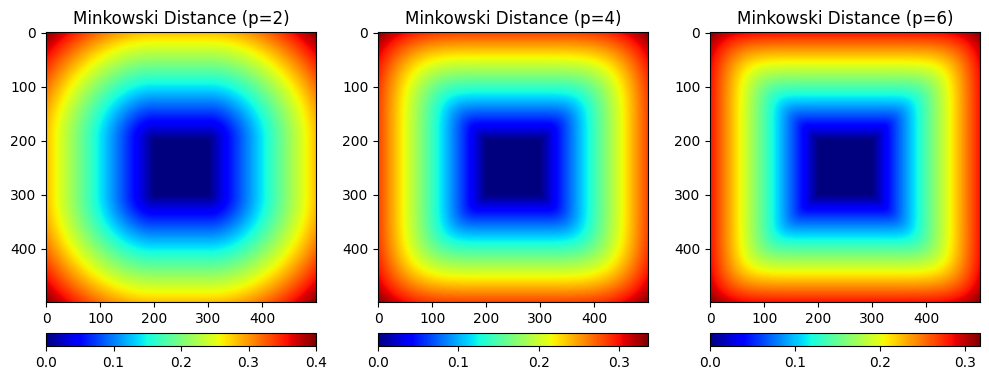
\includegraphics[width=1\linewidth]{images/minkowski.png}
    \caption{(Normalized) Minkowski distance from a central ``target" box for varying values of the exponent $p$ in a 2D space.}
    \label{fig:minkowski}
\end{figure} 



